\section*{3. Problems in Elasticity}
\subsection*{3.2. Formulas}
\subsubsection*{Plane Strain}
On the plane $x$-$y$, the equilibrium and compatibility equations are
\begin{gather*}
    \frac{\partial \sigma_x}{\partial x} + \frac{\partial \tau_{xy}}{\partial y} = 0 \\
    \frac{\partial \sigma_y}{\partial y} + \frac{\partial \tau_{xy}}{\partial x} = 0
    \frac{\partial^2 \sigma_x}{\partial y^2} + \frac{\partial^2 \sigma_y}{\partial x^2} = \frac{\partial^2 \gamma_{xy}}{\partial x \partial y} \\
    \implies \left(\frac{\partial^2}{\partial x^2} + \frac{\partial^2}{\partial y^2}\right) (\sigma_x + \sigma_y) = 0
\end{gather*}
Strain-stress relations are
\begin{align*}
    \epsilon_x &= \frac{1}{E} \left( \sigma_x - \nu \sigma_y \right) \\
    \epsilon_y &= \frac{1}{E} \left( \sigma_y - \nu \sigma_x \right) \\
    \epsilon_z &= -\frac{\nu}{E} \left( \sigma_x + \sigma_y \right) \\
    \gamma_{xy} &= \frac{\tau_{xy}}{G} \\
    \gamma_{xz} &= \gamma_{yz} = 0 
\end{align*}
Stress-strain relations are
\begin{align*}
    \sigma_x &= \frac{E}{1-\nu^2} \left( \epsilon_x + \nu \epsilon_y \right) \\
    \sigma_y &= \frac{E}{1-\nu^2} \left( \epsilon_y + \nu \epsilon_x \right) \\
    \tau_{xy} &= G \gamma_{xy} \\
    \sigma_z &= -\frac{\nu}{1-\nu} \left( \epsilon_x + \epsilon_y \right)
\end{align*}
Airy's stress function $\Phi$ relations
\begin{gather*}
    \nabla^4 \Phi = \frac{\partial^4 \Phi}{\partial x^4} + 2 \frac{\partial^4 \Phi}{\partial x^2 \partial y^2} + \frac{\partial^4 \Phi}{\partial y^4} = 0\\
    \sigma_x = \frac{\partial^2 \Phi}{\partial y^2}, \quad \sigma_y = \frac{\partial^2 \Phi}{\partial x^2}, \quad \tau_{xy} = -\frac{\partial^2 \Phi}{\partial x \partial y}
\end{gather*}
\subsubsection*{Thermalelasticity}
Thermal strain, $\epsilon{t} = \alpha T$, relations by superposition,
\begin{align*}
    \epsilon_x &= \frac{1}{E} \left( \sigma_x - \nu \sigma_y \right) + \alpha T \\
    \epsilon_y &= \frac{1}{E} \left( \sigma_y - \nu \sigma_x \right) + \alpha T \\
    \epsilon_z &= -\frac{\nu}{E} \left( \sigma_x + \sigma_y \right) + \alpha T \\
    \gamma_{xy} &= \frac{\tau_{xy}}{G} 
\end{align*}
Thermal stress relations,
\begin{align*}
    \sigma_x &= \frac{E}{1-\nu^2} \left( \epsilon_x + \nu \epsilon_y \right) - \frac{E\alpha T}{1-\nu} \\
    \sigma_y &= \frac{E}{1-\nu^2} \left( \epsilon_y + \nu \epsilon_x \right) - \frac{E\alpha T}{1-\nu} \\
    \sigma_z &= -\frac{\nu}{1-\nu} \left( \epsilon_x + \epsilon_y \right) - \frac{E\alpha T}{1-\nu} \\
    \tau_{xy} &= G \gamma_{xy} 
\end{align*}
Stress function $\Phi$ relations,
\begin{align*}
    \left(\frac{\partial^2}{\partial x^2} + \frac{\partial^2}{\partial y^2} \right)(\sigma_x + \sigma_y + \alpha ET) &= 0 \\
    \implies \nabla^4 \Phi + \alpha E \nabla^2 T &= 0 
\end{align*}
\subsubsection*{Polar Coordinates}
Displacement-strain relations,
\begin{gather*}
    \epsilon_r = \frac{\partial u}{\partial r}, \quad \epsilon_\theta = \frac{u}{r} + \frac{1}{r} \frac{\partial v}{\partial \theta} \\
    2\epsilon_{r\theta} = \gamma_{r\theta} = \frac{\partial v}{\partial r} - \frac{v}{r} + \frac{1}{r} \frac{\partial u}{\partial \theta}
\end{gather*} 
Strain-stress relations for plane stress,
\begin{gather*}
    \epsilon_r = \frac{1}{E} \left( \sigma_r - \nu \sigma_\theta \right), \quad \epsilon_\theta = \frac{1}{E} \left( \sigma_\theta - \nu \sigma_r \right) \\
    \epsilon_{r\theta} = \frac{1}{2G} \tau_{r\theta} 
\end{gather*}
Airy's stress function $\Phi$ relations,
\begin{gather*}
    \sigma_r = \frac{1}{r}\frac{\partial \Phi}{\partial r} + \frac{1}{r^2} \frac{\partial^2 \Phi}{\partial \theta^2}, \quad \sigma_\theta = 
    \frac{\partial^2 \Phi}{\partial r^2} \\
    \tau_{r\theta} = \frac{1}{r^2}\frac{\partial \Phi}{\partial \theta} - \frac{1}{r}\frac{\partial^2 \Phi}{\partial r \partial \theta} = -
    \frac{\partial}{\partial r} \left( \frac{1}{r} \frac{\partial \Phi}{\partial \theta} \right)
\end{gather*}
Compatibility,
\begin{gather*}
    \nabla^2 \Phi = \frac{\partial^2 \Phi}{\partial r^2} + \frac{1}{r} \frac{\partial \Phi}{\partial r} + \frac{1}{r^2} \frac{\partial^2 \Phi}{\partial \theta^2} \\
    \nabla^4 \Phi = \left(\frac{\partial^2}{\partial r^2} + \frac{1}{r} \frac{\partial}{\partial r} + \frac{1}{r^2} \frac{\partial^2}{\partial \theta^2} \right) 
    \nabla^2 \Phi=0
\end{gather*}
Transformation equations,
\begin{align*}
    \sigma_r &= \frac{1}{2}(\sigma_x + \sigma_y) + \frac{1}{2}(\sigma_x - \sigma_y) \cos{2\theta} + \tau_{xy} \sin{2\theta} \\
    \tau_{r\theta} &= -\frac{1}{2}(\sigma_x - \sigma_y) \sin{2\theta} + \tau_{xy} \cos{2\theta} \\
    \sigma_\theta &= \frac{1}{2}(\sigma_x + \sigma_y) - \frac{1}{2}(\sigma_x - \sigma_y) \cos{2\theta} - \tau_{xy} \sin{2\theta}
\end{align*}
or 
\begin{align*}
    \sigma_x &= \frac{1}{2}(\sigma_\theta + \sigma_r) + \frac{1}{2}(\sigma_r - \sigma_\theta) \cos{2\theta} - \tau_{r\theta} \sin{2\theta} \\
    \tau_{xy} &= -\frac{1}{2}(\sigma_r - \sigma_\theta) \sin{2\theta} + \tau_{r\theta} \cos{2\theta} \\
    \sigma_y &= \frac{1}{2}(\sigma_\theta + \sigma_r) - \frac{1}{2}(\sigma_r - \sigma_\theta) \cos{2\theta} + \tau_{r\theta} \sin{2\theta}
\end{align*}
\subsubsection*{Concentrated Loads}
Wedge of unit thickness, under load $P$, and angle $\alpha$,
\begin{align*}
    \sigma_{r} &= - \frac{P \cos{\theta}}{r(\alpha + \frac{1}{2}\sin{2\alpha})},\quad \sigma_{\theta} = 0, \quad \tau_{r\theta} = 0\\
    \sigma_{x} &= \sigma_{r} \cos^2{\theta} = - \frac{P \cos^4{\theta}}{L(\alpha + \frac{1}{2}\sin{2\alpha})} \\
    \tau_{xy} &= \frac{P\sin\theta \cos^3\theta}{L(\alpha + \frac{1}{2}\sin{2\alpha})} \\
    (\sigma_{x})_{\text{elem}} &= - \frac{P}{2L\tan{\alpha}}
\end{align*}
Note that the normal stress is maximum at $\theta = 0$ and minimum at $\theta = \alpha$. Shear stress is maximum at 
$\theta = \alpha$ if $\alpha < 30^\circ$ and at $\theta = 30^\circ$ if $\alpha \geq 30^\circ$.

If the wedge is a straight boundary, $\alpha = \pi/2$, then
\begin{align*}
    \sigma_r = - \frac{2P\cos\theta}{\pi r}, \quad \sigma_\theta = 0, \quad \tau_{r\theta} = 0
\end{align*}

\begin{figure}[H]
    \centering
    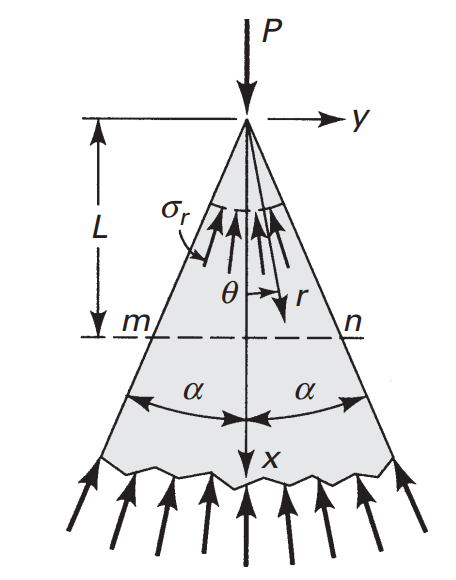
\includegraphics[width=0.3\linewidth]{Figures/sec3 concentrated load P.png}
    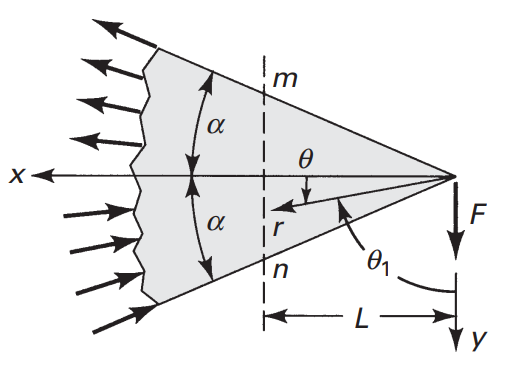
\includegraphics[width=0.4\linewidth]{Figures/sec3 concentrated load side.png}
    \caption{Wedge of unit thickness under load $P$ and $F$ per unit thickness}
    \label{fig:sec3 concentrated load P}
\end{figure}

For bending of a wedge, under load $P$, and angle $\alpha$,
\begin{align*}
    \sigma_{r} &= -\frac{F \cos{\theta_1}}{r(\alpha - 0.5\sin(2\alpha)} = -\frac{F \sin{\theta}}{r(\alpha + 0.5\sin(2\alpha)} \\
    \sigma_{\theta} &= \tau_{r\theta} = 0 \\
    \sigma_x &= \sigma_r \cos^2{\theta} = -\frac{F \sin\theta \cos^2\theta}{r(\alpha + 0.5\sin(2\alpha)} \\
    \sigma_y &= \sigma_r \sin^2{\theta} = -\frac{F \sin^3\theta}{r(\alpha + 0.5\sin(2\alpha)} \\
    \tau_{xy} &= \sigma_r \sin\theta \cos\theta = -\frac{F \sin^2\theta \cos\theta}{r(\alpha + 0.5\sin(2\alpha)} \\
    (\sigma_{x})_{\text{elem}} &= -\frac{F}{2r\tan\alpha}
\end{align*}

So for a combined load $P$ and $F$,
\begin{align*}
    \sigma_r &= -\frac{P \cos{\theta}}{r(\alpha + 0.5\sin(2\alpha)} -\frac{F \sin{\theta}}{r(\alpha + 0.5\sin(2\alpha)} \\
    \sigma_{\theta} &= \tau_{r\theta} = 0 
\end{align*}


\subsubsection*{Stress Concentrations}
For stress concentration factor $K$,
\begin{align*}
    K = \frac{\sigma_{\text{max}}}{\sigma_{\text{nom}}}
\end{align*}
For circular hole in a large plate in tension stress $\sigma_o$,
\begin{align*}
    (\sigma_{\theta})_{\text{max}} &= 3 \sigma_o, \quad \theta = \pm \pi/2 \\
    (\sigma_{\theta})_{\text{min}} &= - \sigma_o, \quad \theta = 0, \pm \pi
\end{align*}
For tension $\sigma_{ox}$ and $\sigma_{oy}$,
\begin{align*}
    (\sigma_{\theta})_{\text{max}, x} &= 3 \sigma_{ox} - \sigma_{oy}, \quad \theta = \pm \pi/2 \\
    (\sigma_{\theta})_{\text{min}, y} &= 3 \sigma_{oy} - \sigma_{ox}, \quad \theta = 0, \pm \pi
\end{align*}
\begin{figure}[H]
    \centering
    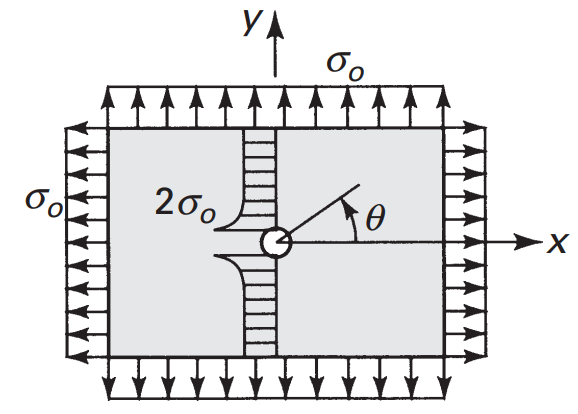
\includegraphics[width=0.3\linewidth]{Figures/sec3 hole in large plate.png}
    \caption{Stress concentration factor for circular hole in a large plate (10/10 figure)}
    \label{fig:sec3 stress concentration for circular hole in large plate}
\end{figure}
